% !TEX root = ../main.tex

\chapter{Background}

This chapter aims to provide an understanding of the project and its background, and the technologies that are used in relation to this project.

\section{Sentiment Analysis}

Sentiment Analysis, also known as opinion mining, may be defined as the process of analysis text in order to find the opinion of an author about a topic\cite{feldman2013techniques}. A text will contain objective facts, however, it will also contain the opinions and feelings of the author in regards to the topic at hand. It is quite hard for computers to analyse a given text for sentiment, as it does not come naturally unlike for humans. For this reason, a series of tools and techniques are being developed in order to facilitate this process. These techniques draw from different areas of knowledge, including natural language processing, and various statistical and machine learning classification techniques. There has been a large amount of research into sentiment analysis, since the information that may be extracted can be of great value. This may be for analysing how a ompany is doing, as well as how a politicians image is progressing. Given that this information can be important for the financial status of a company, there has been a large amount of investment into this field. However, there is still a large amount to learn.

\subsection{Overview}

As may be seen in figure \ref{fig:sentStructure}, there is a general structure any system attempting to analyse sentiment will follow. That is it will gather a corpus of texts from a given source. It will process them in the appropriate manner to gather the correct meta-data. alongside some linguistic resources and/or lexicons it will analyse the documents, and draw sentiment scores for the various aspects being analysed. The discussion of the technicalities of the design and implementation of these components is executed up will be discussed in the appropriate chapters.

\begin{figure}[h!]
    \centering
    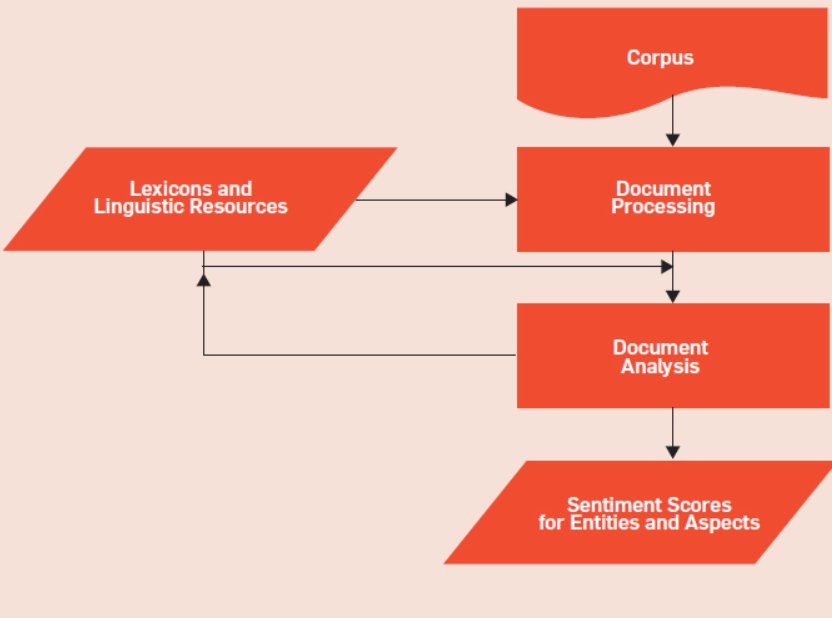
\includegraphics[width=15cm,height=7cm,keepaspectratio]{background/sentStructure.png}
    \caption{General Sentiment Analyser Structure\cite{feldman2013techniques}}
    \label{fig:sentStructure}
\end{figure}

The topic of how the analysis itself is conducted on the texts should be discussed. As shown in the referenced paper\cite{feldman2013techniques}. It may be proken down into 4 distinct methods:
\begin{itemize}
    \item Document Level Sentiment Analysis -- assumes the document contains an opinion on one main object. There are two main approaches for analysis in this manner:
    \begin{itemize}
        \item Supervised Learning -- assumes there is a finite set of classes the document may be classified into. In the simplest case: positive, negative and neutral.
        \item Unsupervised Learning -- determines the sematic orientation of specific phrases in the document. If the average semantica orientation is over a specific threshold, the document is deemed positive, otherwise it is deemed negative. There are two main approaches towards selecting a phrase:
        \begin{itemize}
            \item A predefined Part of Speech pattern\cite{wilson-etal-2005-recognizing}
            \item A lexicon of sentiment words and phrases\cite{10.1162/COLI_a_00049}
        \end{itemize}
    \end{itemize}
    \item Sentence Level Sentiment Analysis -- a document may contain multiple opinions on the same object. It is assumed that the identity of the object discussed in each sentence is known, and there is a single opinion in each sentence. The sentences must be determined to be subjective or objective, as only subjective sentences will be analysed. A supervised method is usually used to classify the sentences\cite{10.3115/1119355.1119372}. Once this fact is determined the appropriate sentences can then be analysed, similarly to how it is done at the document level\cite{analysePredictiveOpinionsWeb,10.3115/1119355.1119372}.
    \item Aspect Based Sentiment Analysis -- a given sentence may discuss various aspects, and each aspect may have a different opinion associated to it. The research problem here is the ability to identify aspects, both explicit and implicit. Once these are identified they are classified by similar means as before.
    \item Comparative Sentiment Analysis -- opinions may be in relation to an opinion of a similar object. This method is used to identify the preferred object between the ones compared. It is important in this method to remove sentences without a comparative opinion\cite{analysePredictiveOpinionsWeb}.
\end{itemize}

A problem which occurs when attempting to execute on any of these methods is Sentiment Lexicon Aquisition. this is a most crucial resource. There are three main approaches for solving this:
\begin{itemize}
    \item Manually -- it is a laborious and prohibitive effort, especially considering each domain requires its own lexicon
    \item Dictionary-Based -- starts with a small set of seed words, and uses synonyms and antonyms in orde to expand itself. The acquired lexicon will be domain independent\cite{sentimentDictoinaryConstruction,kamps-etal-2004-using,Peng_Park_2011}.
    \item Corpus-Based -- Methods based on this proposition use the corpus of texts to identify acquire the lexicon. An example of a corpus-based method is the following. Identify a list of adjectives with a known polarity. Use linguistic connectors such as AND and OR in order to attach a polarity to adjectives connected to known adjectives by these words within the corpus\cite{hatzivassiloglou-mckeown-1997-predicting,opinionWordExpansion}.
\end{itemize}

\subsection{Financial Sentiment Analysis}

Using sentiment analysis in a financial context has a significant history. A paper from 1971\cite{RePEc:ucp:jnlbus:v:44:y:1971:i:2:p:193-219} even analysed twenty years worth of New York Times headlines to see how market reacted to positive and negative news. Interestingly he found that markets do react to both types of news, however, they react to negative news in a more pronounced and long term manner.

It is important to note that when analysis sentiment, the use of meta-data analysis is employed alongside the analysis of sentiment itself. An example of this would be the use of volume of articles in a given timeperiod.

An often cited paper in this area is one written by Tetlock et al\cite{RePEc:bla:jfinan:v:63:y:2008:i:3:p:1437-1467}. This paper worked with articles classified as negative or positive as well as the tallying of sentiment terms with an article. It used the Dows Jones News Service and the Wall Street Journal from 1984 to 2004 as new sources. The General Inquirer method was used to count the positive and negative terms, as well as a self-defined lexicon associated with a firm. It used term frequency and z-score when analysing the output in simple regression models. The main findings were that stock did react badly to negative news about the firm, even more so if the document contained a high frequency of words from the firm specific lexicon.

\subsection{Sentiment Proxy}

The text compiled are from newspapers, magazines, etc. These are known as sentiment proxies. Proxy may be defined as the authority to represent someone else. What this means is that the sentiment extracted is not the market sentiment, however, it is an indicator or proxy of it.

\section{Financial Data Acquisition}

The are various methods that may be employed when attemptivng to retrieve financial data for a company. The goal is to obtained the desired financial data over the required time period. This is a relatively straight-forward process given the wides-spread availability of third party services as has been done already, such as APIs\cite{hochreiter2015computing}.

\section{System Structure}

Stock market analysis is a heavily researched area, as it allows the creation of a large amount of value. It creates a large amount of information on a regular , and this is considered very valuable for investors as well as academics. There have been numerous attempts at attempting to estimate the future growth of a stock given the information provided by the market\cite{khedr2017predicting,pagolu2016sentiment,nti2020predicting}. These examples can be used in order to study the approaches and adapt them to this project. There have been studies relying on social media information analysis\cite{3f9f26dccdd44d8e9791959e44112b4b} as well as news analysis\cite{Uhr2014SentimentAI}. These studies utilise various natural language processing techniques, as well as data mining techniques to analyse their sources. They then use machine learning models in order to create an estimation for the level of market returns. One paper\cite{7e2040917a3f4f90a22d23d66e18f6f8} even used hourly stock prices alongside tweets in order to estimate the direction of the stock price within the next hour. These studies were analysed for the methodology in which they collected, and made their analysis. These were useful for creating a design which would handle the data appropriately in order to gather it and analyse it appropriately. An example of a structure given in one of these papers\cite{khedr2017predicting}, as seen in figure \ref{fig:exStructure}.

\begin{figure}[h!]
    \centering
    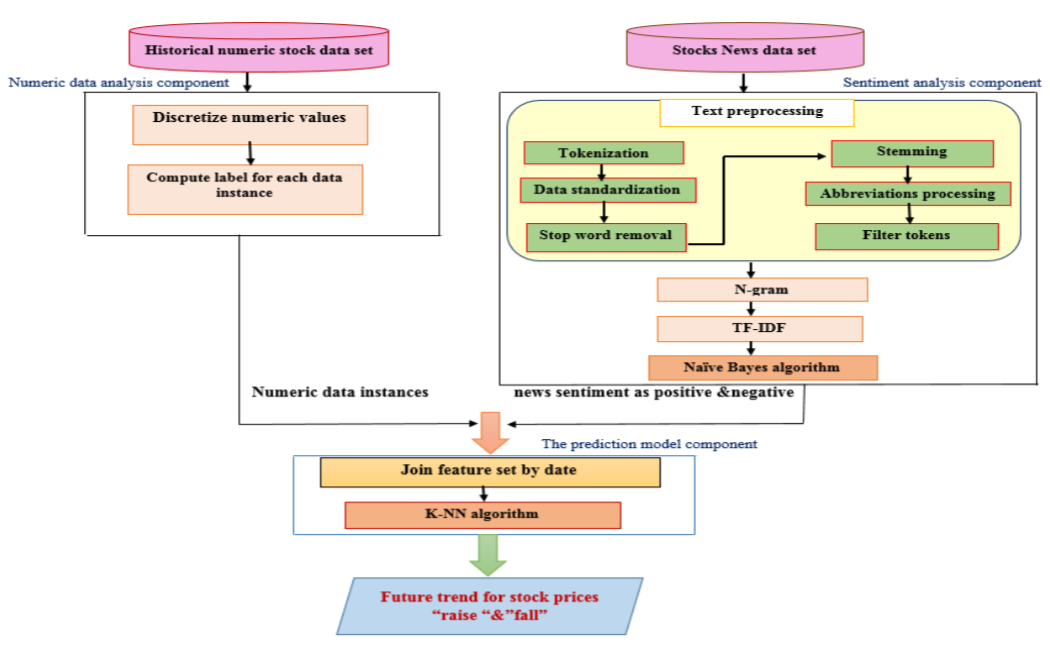
\includegraphics[width=15cm,height=7cm,keepaspectratio]{background/exStructure.png}
    \caption{Example Structure of Estimator\cite{khedr2017predicting}}
    \label{fig:exStructure}
\end{figure}

From this, the idea of having a component for each data source, as well as having at least one data source for price values and one for sentiment values can be taken. It is also understood that some processing of the data is required in order to function within the analysis. All of the data-sets must be joined together in such a way that they may all be used in tandem.

\section{Machine Learning Models}

In order to make estimations from the price and sentiment values there was an exploration of various machines learning models. It has been seen that estimating returns from sentiment has been explored in the past\cite{khedr2017predicting}.

There were various models explored within this system. The following models were all chosen because they are various different different models which are excellent at classifications. They each have different strength and weaknesses, and for that reason one the models may work better or worse depending on the dataset.
\begin{itemize}
    \item \texttt{KNeighborsClassifier (KNN)} -- KNN is a non-parametric and lazy learning algorithm. Non-parametric means there is no assumption for underlying data distribution. In KNN, K is the number of nearest neighbors. The number of neighbors is the core deciding factor. What this means is that the decision for the output will be based on the k nearest neighbours. K is determined through hyperparameter training as described above\cite{knnClass}.
    \begin{figure}[h!]
        \centering
        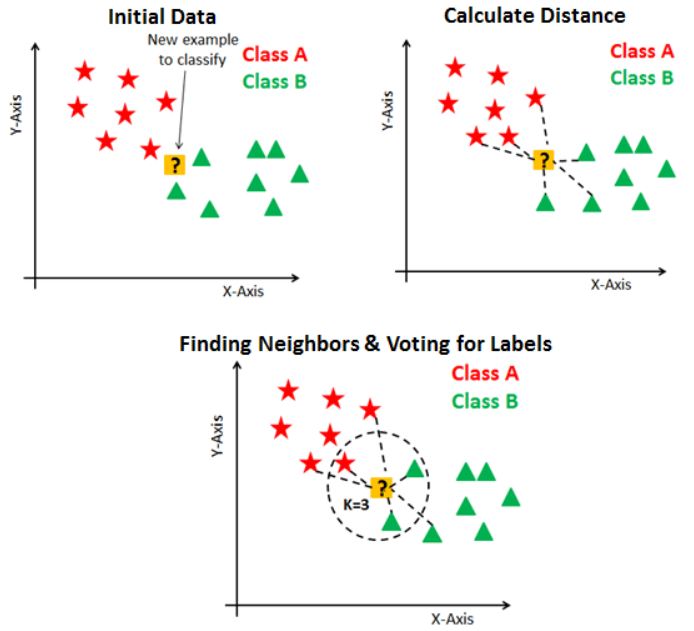
\includegraphics[width=15cm,height=5cm,keepaspectratio]{implementation/kNN.png}
        \caption{KNeighborsClassifier}
        \label{fig:kNN}
    \end{figure}
    \item \texttt{DecisionTreeClassifier} -- A decision tree is created from the training data in order to achieve the classification. A decision tree is a flowchart-like tree structure where an internal node represents a feature, the branch represents a decision rule, and each leaf node represents the outcome. This can be seen in the figure below\cite{decisionTreeClass}.
    \begin{figure}[h!]
        \centering
        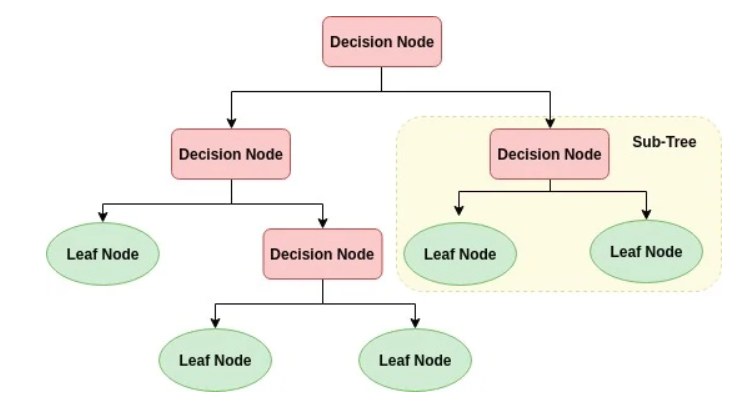
\includegraphics[width=15cm,height=5cm,keepaspectratio]{implementation/decisionTree.png}
        \caption{Decision Tree}
        \label{fig:decisionTree}
    \end{figure}
    Within the system the \verb|DecisionTreeClassifier()| class is created. However to quickly cover the steps in creating a decision tree, they are the following:
    \begin{enumerate}
        \item Select the best feature using Attribute Selection Measures to split the dataset. Attribute selection measure is a heuristic for selecting the splitting criterion that partition data into the best possible manner. Attribute Selection Measure provides a rank to each feature by explaining the given dataset. There are multiple ways of assigning each feature a value. Some of these being:
        \begin{itemize}
            \item \texttt{Information Gain} -- It computes the difference between entropy before split and average entropy after split of the dataset based on given attribute values
            \item \texttt{Gain Ratio} -- It extends Information Gain by handling the issue of bias by normalizing the information gain using Split Info
        \end{itemize}
        \item Make that feature a decision node and breaks the dataset into smaller subsets.
        \item Starts tree building by repeating this process recursively for each child until one of the condition will match:
        \begin{itemize}
            \item All the tuples belong to the same feature value.
            \item There are no more remaining features.
            \item There are no more instances.
        \end{itemize}
    \end{enumerate}
    \item \texttt{GaussianProcessClassifier} -- It is a classifier which uses Gaussian Processes. Gaussian Processes are a generalization of the Gaussian probability distribution. They are a type of kernel model capable of predicting highly calibrated class membership probabilities, although the choice and configuration of the kernel used at the heart of the method can be challenging. For the purposes of this project an arbitrarily chosen kernel configuration was chosen in order to simplify the process. The choice was the basic confugration shown in the documentation for the class. A radial basis function was used to create this.  A radial basis function being a real-valued function whose value depends only on the distance between the input and some fixed point. For further explanation, the documentation for this can be referenced\cite{gaussProcessClass}.
    \item \texttt{AdaBoostClassifier} -- AdaBoost or Adaptive Boosting is a type of ensemble boosting classifier. Boosting algorithms are a set of weak classifiers which create a strong classifier. These algorithms help decrease model bias. The basic concept behind Adaboost is to set the weights of classifiers and training the data sample in each iteration such that it ensures the accurate predictions of unusual observations. The general steps for this classifier are\cite{adaBoostClass}:
    \begin{enumerate}
        \item Initially, all observations are given equal weights
        \item A model is built on a subset of data
        \item Using this model, predictions are made on the whole dataset
        \item Errors are calculated by comparing the predictions and actual values
        \item While creating the next model, higher weights are given to the data points which were predicted correctly
        \item Weights can be determined using the error value. For instance, the higher the error the more is the weight assigned to the observation
        \item This process is repeated until the error function does not change, or the maximum limit of the number of estimators is reached
    \end{enumerate}
    \item \texttt{RandomForestClassifier} -- This algorithm creates decision trees on randomly selected data samples, gets a prediction from each tree and selects the best solution by means of voting. The n hyper parameter must be trained, this determines the number of forests to use, i.e. the number of random samples. The general steps are\cite{randomForestClass}:
    \begin{enumerate}
        \item Select random samples from a given dataset
        \item Construct a decision tree for each sample and get a prediction result from each decision tree
        \item Perform a vote for each predicted result
        \item Select the prediction result with the most votes as the final prediction
    \end{enumerate}
    \begin{figure}[h!]
        \centering
        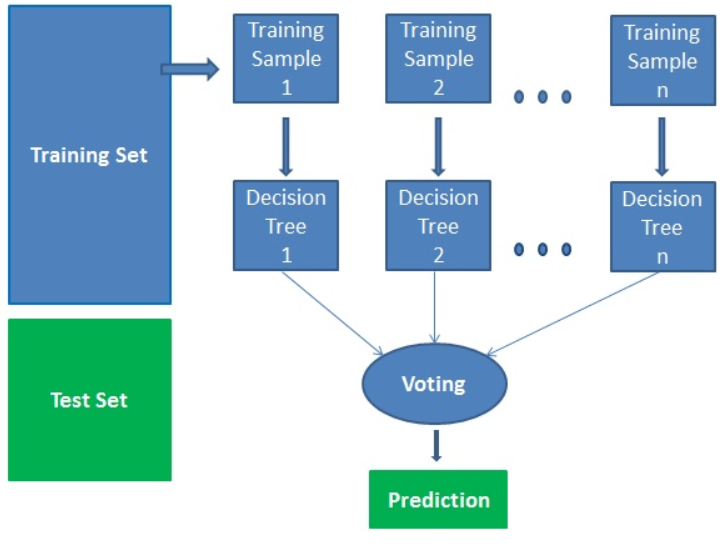
\includegraphics[width=15cm,height=7cm,keepaspectratio]{implementation/randomForest.png}
        \caption{RandomForestClassifier}
        \label{fig:randomForest}
    \end{figure}
\end{itemize}

\section{Statistical Tools}

Given that this paper is exploring statistical relationships, an understanding of the statistical and econometric tools used is quite important.

\paragraph{Descriptive Statistics}

When describing a dataset descriptive statistics may be used. The following statistics are used in many cases:
\begin{itemize}
    \item \texttt{Mean} -- The average of all the data-points
    \item \texttt{Standard Error} -- Measures the accuracy with which a sample distribution represents a population by using standard deviation
    \item \texttt{Median} -- The value separating the higher half from the lower half of a data-set
    \item \texttt{Mode} -- The most common value in the data-set
    \item \texttt{Standard Deviation} -- Measures the amount of variation or dispersion of the data-points
    \item \texttt{Sample Variance} -- The average of the squared differences from the mean, helps measure variance within the data-points
    \item \texttt{Kurtosis} -- Defines how heavily the tails of a distribution differ from the tails of a normal distribution, i.e. it measures the number of extreme values in the data-set
    \item \texttt{Skewness} -- Measures the asymmetry of the distribution about its mean
    \item \texttt{Range} -- The difference between the maxim and minimum values
    \item \texttt{Minimum} -- The minimum value found in the data-points
    \item \texttt{Maximum} -- The maximum value found in the data-points
    \item \texttt{Sum} -- The sum of the data-points
    \item \texttt{Count} -- The number of data-points analysed
\end{itemize}

\paragraph{Correlation}

It is any statistical relationship, whether causal or not, between two random variables or bivariate data. It commonly refers to the degree to which a pair of variables are linearly related. It can indicate a predictive relationship. The method of calculating correlation is the Pearson correlation coefficient, which is sensitive only to a linear relationship between two variables (which may be present even when one variable is a non-linear function of the other). Other, more robust, correlation coefficients have been developed, for example Spearman's rank correlations, meaning they are more sensitive to non-linear relationships.

\paragraph{Autocorrelation}

It is the correlation of a variable with an offset copy of itself. In the context of time series, it is the similarity between observations as a function of the time lag between them.

\paragraph{Augmented Dickey-Fuller Test}

It tests the null hypothesis that a unit root is present in a time series sample. It is an augmented version of the Dickey–Fuller test for more a complex time series data-set. It is used to identify whether the data-set can be consistently described no matter the sub-set chosen, assuming the subset is random.

\paragraph{Vector Autoregression (VAR)}

It is a statistical model which captures the relationship between series of quantities as they change over time\cite{varDairy}. VAR models allow for multi-variate timeseries, thus generalising the uni-variate autoregressive model.

\section{Additional Mechanisms}

\paragraph{Efficient Market Hypothesis}

It hypothesises that stock prices reflect all available information. This implies that it is impossible to "beat the market" in a consistent manner on a risk-adjusted basis since market prices should only react to new information\cite{malkiel1989efficient}. Three levels of market efficiency have been hypothesised:
\begin{itemize}
    \item Weak -- Asserts that prices reflect the information contained in the historical sequence of prices.
    \item Semi-Strong -- Asserts that prices reflect historical price information as well as publicly available information relevant to the company's securities.
    \item Strong -- Asserts that prices reflect all information known to any market participant.
\end{itemize}

\paragraph{Mean Reversion}

Mean reversion assumes that a stock's returns eventually revert to their long-term mean\cite{POTERBA198827}. It is assumes there is a certain amount of variance to the accuracy of the market price, indicating that the market is not fully rational. This noise has been researched\cite{fischerNoise}, and some sources have been identified such as naive traders, information asymmetry, etc. A naive trader is one that makes irrational decisions given the information available, that is they may make trades based on a gut feeling for example. This is unlike an informed trader which maes rational decisions. Some important research into the subject matter was done by Bachelier\cite{bachelier1900theorie}, which posites that there is Brownian motion within market prices, i.e. there is a certain amount of implied volatility.

\paragraph{Fashions}

It is important to mention the contribution of fashions in the financial context. This refers to when traders follow the crowd with their investment decisions, this is also known as herding. This generally categorises trades that a trader would not have made, except for the fact that they heard of a number of trader which made the investment. Herd behaviour is a bias studied in behavioural psychology\cite{conformity}, which is generally considered useful for humans, however, it may become counter-productive in the financial sector. Sentiment relates to this by creating an initial push which, if large enough, may override even the sensibilities of an informed trader. This may lead to the creation of a bubble, which is a set of short term gains that will lead to a long-term crash.

\paragraph{Feedback}

Another item that effect the market is the potential feedback loop created between sentiment and prices. That is sentiment may effect the performance of the market, however, the performance may then influence sentiment.

\paragraph{Bias}

Senders of sentiment, for example journalists may have a bias towards a specific company which will influence the way articles are written. The same can be said for receivers, that is they may intepret a given article differently depending on their initial biases, and therefore make diffrent choices.

\section{Background Summary}

The chapter provides background details necessary to understand the project.